%%%%%%%%%%%%%%%%%%%%%%%%%%%%%%%%%%%%%%%%
% Beamer Presentation
% LaTeX Template
% Version 1.0 (10/11/12)
%
% This template has been downloaded from:
% http://www.LaTeXTemplates.com
%
% License:
% CC BY-NC-SA 3.0 (http://creativecommons.org/licenses/by-nc-sa/3.0/)
%
%%%%%%%%%%%%%%%%%%%%%%%%%%%%%%%%%%%%%%%%%

%----------------------------------------------------------------------------------------
%	PACKAGES AND THEMES
%----------------------------------------------------------------------------------------

\documentclass[xcolor=dvipsnames, aspectratio=169]{beamer}

\mode<presentation> {

% The Beamer class comes with a number of default slide themes
% which change the colors and layouts of slides. Below this is a list
% of all the themes, uncomment each in turn to see what they look like.

\usetheme{Madrid} %Hannover
% As well as themes, the Beamer class has a number of color themes
% for any slide theme. Uncomment each of these in turn to see how it
% changes the colors of your current slide theme.
\useoutertheme{infolines} % Alternatively: miniframes, infolines, split
\useinnertheme{circles}
\definecolor{UBCblue}{rgb}{0.04706, 0.13725, 0.26667} % UBC Blue (primary)
\usecolortheme[named=UBCblue]{structure}
}

\usepackage{graphicx} % Allows including images
\usepackage{booktabs} % Allows the use of \toprule, \midrule and \bottomrule in tables
\usepackage{textpos}
\usepackage{caption}
\usepackage[utf8]{inputenc}
\usepackage[brazilian]{babel}
\usepackage{csquotes}
\usepackage{listings}
\setbeamertemplate{caption}[numbered]
\usepackage[style=abnt]{biblatex}
\addbibresource{bibliography.bib}
\PassOptionsToPackage{useregional}{datetime2}
\usepackage{xcolor}


\definecolor{codegreen}{rgb}{0,0.6,0}
\definecolor{codegray}{rgb}{0.5,0.5,0.5}
\definecolor{codepurple}{rgb}{0.58,0,0.82}
\definecolor{backcolour}{rgb}{0.95,0.95,0.92}
\definecolor{string-color}{rgb}{0.3333, 0.5254, 0.345}

\lstdefinestyle{mystyle}{
    backgroundcolor=\color{backcolour},   
    commentstyle=\color{codegreen},
    keywordstyle=\color{string-color},
    keywordstyle=[2]{\color{codepurple}},
    keywordstyle=[3]{\color{magenta}},
    numberstyle=\tiny\color{codegray},
    stringstyle=\color{codepurple},
    basicstyle=\ttfamily\footnotesize,
    breakatwhitespace=false,         
    breaklines=true,                 
    captionpos=b,                    
    keepspaces=true,                 
    numbers=left,                    
    numbersep=5pt,                  
    showspaces=false,                
    showstringspaces=false,
    showtabs=false,                  
    tabsize=2,
    otherkeywords = {tf, Sequential, SimpleRNN, Dense, GRU, LSTM},
    morekeywords = [3]{keras},
}

\lstset{style=mystyle}
\newcommand{\source}[1]{\vspace{-20pt} \caption*{ Fonte: {#1}} }
\usepackage{copyrightbox}


\makeatletter
% \beamer@nav@subsectionstyle{hide/hide/hide}
\addtobeamertemplate{sidebar left}{%
\hspace{0.5cm}
\includegraphics[width=0.9cm, keepaspectratio]{figures/_brasao_ufsm_cor.png}
% \hspace{2.3cm}
\includegraphics[width=0.8cm, keepaspectratio]{figures/brasao_ctism.png}
% \hspace{2.3cm}\includegraphics[width=1.5cm, keepaspectratio]{_logosbc.png}
% \hspace{2.3cm}\includegraphics[width=1.5cm, keepaspectratio]{_logoERRC.png}%
}{}


\setbeamertemplate{footline}
{
	\leavevmode%
	\hbox{%
	    % \hspace{0.5cm}
\includegraphics[width=0.8cm, keepaspectratio]{figures/_brasao_ufsm_cor.png}
		\begin{beamercolorbox}[wd=.333333\paperwidth,ht=2.25ex,dp=1ex,right]{date in head/foot}%
			\usebeamerfont{date in head/foot}\insertshortdate{}\hspace*{2em}
			\insertframenumber{} / \inserttotalframenumber\hspace*{2ex} 
		\end{beamercolorbox}}%
		%\vskip0pt%
	}
\makeatother

%----------------------------------------------------------------------------------------
%	TITLE PAGE
%----------------------------------------------------------------------------------------

\title[Proximity Sensors]{Proximity Sensors} % The short title appears at the bottom of every slide, the full title is only on the title page

\author[FDR]{Fábio Demo da Rosa} % Your name
%\includegraphics[]{logositeredes.png}
\institute[UFSM] % Your institution as it will appear on the bottom of every slide, may be shorthand to save space
{
Universidade Federal de Santa Maria \\ % Your institution for the title page
Pós-Graduação em Ciência da Computação \\
Disciplina de Robótica Móvel\\
\medskip
\textit{faberdemo@gmail.com} % Your email address
}
\date{\today} % Date, can be changed to a custom date
\newcounter{saveenumi}
\newcommand{\seti}{\setcounter{saveenumi}{\value{enumi}}}
\newcommand{\conti}{\setcounter{enumi}{\value{saveenumi}}}

\resetcounteronoverlays{saveenumi}


\begin{document}

\begin{frame}
\titlepage % Print the title page as the first slide
\end{frame}

\begin{frame}
\frametitle{Visão Geral} %\includegraphics[]{logositeredes.png}} % Table of contents slide, comment this block out to remove it
\tableofcontents % Throughout your presentation, if you choose to use \section{} and \subsection{} commands, these will automatically be printed on this slide as an overview of your presentation
\end{frame}

%----------------------------------------------------------------------------------------
%	PRESENTATION SLIDES
%----------------------------------------------------------------------------------------

%------------------------------------------------
\section[Proximity Sensors]{Proximity Sensors} 
%------------------------------------------------
\begin{frame}[allowframebreaks, fragile]
\frametitle{Proximity Sensors}
	\begin{itemize}
		\item Usados para determina a presença de objetos próximos;
		\item Desenvolvidos para alcance de detecção além do acessível por contato direto ou sensores táteis;
		\item Possuem uma confiabilidade alta;
		\begin{itemize}
			\item Sendo úteis para operações em ambientes adversos;
			\item Alguns desses sensores conseguem suportar impacto e vibração \cite{everett1995sensors}:
			\begin{itemize}
				\item Forças de até 30000 Gs;
				\item Pressão de até 20000 psi.
			\end{itemize}
		\end{itemize}
	\end{itemize}
\end{frame}


%------------------------------------------------
\section[Magnetic Proximity Sensors]{Magnetic Proximity Sensors} 
%------------------------------------------------
\begin{frame}[allowframebreaks, fragile]
\frametitle{Magnetic Proximity Sensors}
	\begin{itemize}
		\item Aplicações \cite{baumermagnetic}:
		\begin{itemize}
			\item Monitoramento das posições finais dos estabilizadores telescópicos;
			\item Limitação do curso em cilindros hidráulicos;
			\item Detecção do nível de líquido utilizando um imã transportado por um flutuador.
		\end{itemize}
		\item Magnetic Reed Switches:
		\begin{itemize}
			\item A forma mais simples de sensor de proximidade magnética;
			\item Possuem vantagens, mas podem ser lentos, propensos a falhas e sensíveis à vibração. 
			\item Reagem apenas a ímãs magnetizados axialmente, requerindo uma elevada força magnética.
			\begin{figure}
                \centering
                \copyrightbox[b]{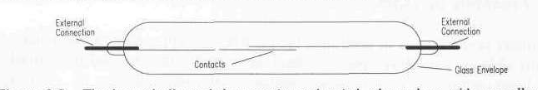
\includegraphics[scale=0.5]{figures/1_reed_switch.png}}%
                {Fonte: \cite{everett1995sensors}}
                \caption{\textit{Reed Switch}, é hermeticamente selado, demonstrado com seus contatos abertos.\\ O tubo é preenchido por um gás inerte para evitar a oxidação dos contatos.}
                \label{fig:1_reed_switch}
            \end{figure}
		\newpage
		\end{itemize}
		\item Hall Effect Sensors:
		\begin{itemize}
			\item Detectam a presença utilizando a magnitude do campo magnético criado por um objeto;
			\item O princípio do efeito Hall é utilizado para detetar a presença e a intensidade de um campo magnético;
			\item Possuem um alcance de cerca de 0-40mm \cite{fenghalleffect}
			\begin{itemize}
				\item Dependendo diretamente da densidade do fluxo magnético do objeto.
				\item Os ímãs mais fortes têm mais influência e podem acionar o sensor a uma distância relativamente maior.
			\end{itemize}
			\begin{figure}
                \centering
                \copyrightbox[b]{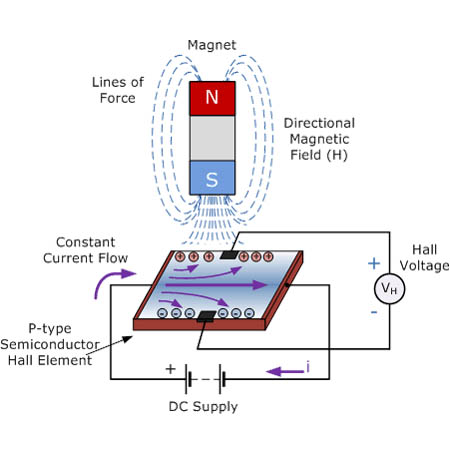
\includegraphics[scale=0.32]{figures/2_Hall-Effect-Proximity-Sensors-02.jpg}}%
                {Fonte: \cite{fenghalleffect}}
                \caption{\textit{Hall Effect Sensor}, onde um ímã é colocado próximo a esse semicondutor fino, \\ ele interrompe o fluxo de corrente desviando os portadores de carga no semicondutor.}
                \label{fig:2_hall_effect_switch}
            \end{figure}
		\end{itemize}
		\item Magnetic Reed Switches:
		\begin{itemize}
			\item O elemento magnético-resistivo é feito de um material especial que reage apenas a campos magnéticos;
			\begin{itemize}
				\item Por exemplo um ímã permanente
			\end{itemize} 
			\item Consegue detectar mesmo campos magnéticos muito fracos;
			\begin{itemize}
				\item O elemento magnético-resistivo é aproximadamente dez vezes mais sensível do que um elemento Hall, o que permite uma grande distância de comutação.
			\end{itemize}
			\item Os interruptores de proximidade magnéticos são omnipolares, o que significa que tanto o pólo norte como o pólo sul estão a ser detectados.
		\end{itemize}
	\end{itemize}
\end{frame}


%------------------------------------------------
\section[Inductive Proximity Sensors]{Inductive Proximity Sensors} 
%------------------------------------------------
\begin{frame}[allowframebreaks, fragile]
\frametitle{Inductive Proximity Sensors}
	\begin{itemize}
		\item Em 1993, eram os mais utilizados em aplicações industriais, para detecção de metais ferrosos e não-ferrosos \cite{everett1995sensors};
		\item Geram um campo eletromagnético ocilatório (100Khz até 1 MHz);
		\begin{figure}
			\centering
			\copyrightbox[b]{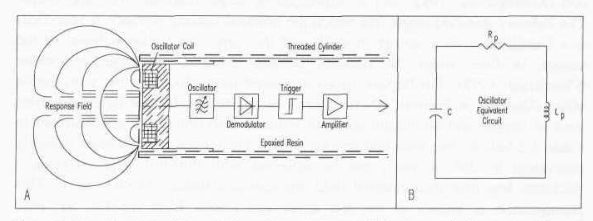
\includegraphics[scale=0.6]{figures/3_diagram_proximity_sensor.png}}%
			{Fonte: \cite{everett1995sensors}}
			\caption{Diagrama do \textit{proximity sensor} tipo ECKO e o circuito de oscilador equivalente.}
			\label{fig:3_diagram_proximity_sensor}
		\end{figure}
		\newpage
		\item O comparador de limite alterna de um estado desligado para um estado ligado.
		\begin{figure}
			\centering
			\copyrightbox[b]{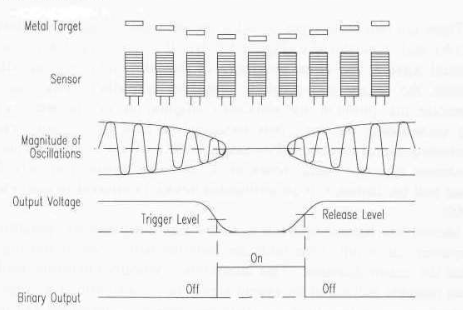
\includegraphics[scale=0.6]{figures/4_inductive_sensor.png}}%
			{Fonte: \cite{everett1995sensors}}
			\caption{Uma pequena diferença entre os níveis de disparo e liberação (histerese) elimina a instabilidade da saída à medida que o alvo entra e sai do alcance.}
			\label{fig:4_inductive_sensor}
		\end{figure}
		\item Um exemplo de uso envolve um grande manipulador industrial que limpa os cascos externos de navios em doca seca com abrasivo de aço. 
		\begin{itemize}
			\item Três sensores indutivos analógicos são usados para detectar a presença da superfície do casco de aço.
		\end{itemize}
		\begin{figure}
			\centering
			\copyrightbox[b]{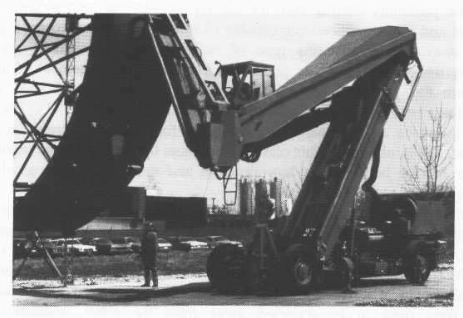
\includegraphics[scale=0.43]{figures/5_robotic_shot_blasting_device_ship.png}}%
			{Fonte: \cite{everett1995sensors}}
			\caption{esse dispositivo robótico de jateamento com granalha de aço usa sensores de proximidade para manter o efetor de ciclo fechado em contato vedado com o casco do navio.}
			\label{fig:5_robotic_shot_blasting_device_ship}
		\end{figure}
	\end{itemize}
\end{frame}

%------------------------------------------------
\section[Capacitive Proximity Sensors]{Capacitive Proximity Sensors} 
%------------------------------------------------
\begin{frame}[allowframebreaks, fragile]
\frametitle{Capacitive Proximity Sensors}
	\begin{itemize}
		\item Ao contrário dos sensores anteriores, os sensores capacitivos detectam mais que alvos metálicos \cite{everett1995sensors};
		\begin{itemize}
			\item Podem detectar materiais dielétricos (isolantes).
		\end{itemize}
		\item Efetivos para aplicações de curto-alcance até alguns pés de distância;
		\item Reagem a variação na capacitância elétrica entre o sensor (ou placa) e o redor do seu alvo;
		\begin{itemize}
			\item Ao objeto se aproximar, a mudança na geometria ou nas caracterísitca dielétricas aumentam a capacitância.
		\end{itemize}
		\item Na Figura \autoref{fig:6_capaciflector}, podemos observa um sensor desenvolvido pela NASA com enfoque em prevenção de colisão robótica \cite{everett1995sensors};
		\begin{itemize}
			\item Onde braços robóticos manipuladores (em aplicações industriais e espaciais), capazes de detectar a presença humana a uma distância de até 30,48 cm.		\end{itemize}
		\begin{figure}
			\centering
			\copyrightbox[b]{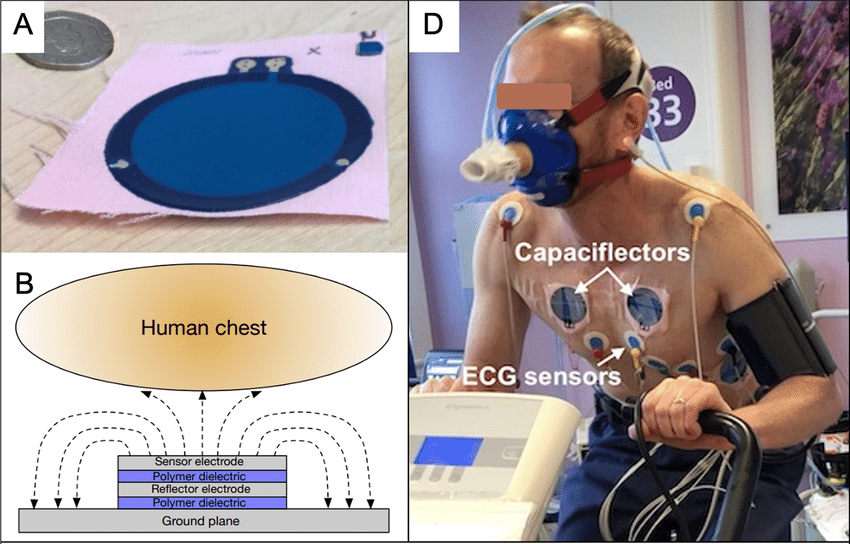
\includegraphics[scale=0.9]{figures/6_The-capaciflector-as-a-respiratory-rate-RR-sensor-A-Photograph-showing-one-printed.png}}%
			{Fonte: \cite{hayward2022capaciflector}}
			\caption{Capaciflector utilizado em outro estudo, com enfoque em medição da taxa respiratória.}
			\label{fig:6_capaciflector}
		\end{figure}
	\end{itemize}
\end{frame}


%------------------------------------------------
\section[Ultrasonic Proximity Sensors]{Ultrasonic Proximity Sensors} 
%------------------------------------------------
\begin{frame}[allowframebreaks, fragile]
\frametitle{Ultrasonic Proximity Sensors}
	\begin{itemize}
		\item O sensor ultrasônico de proximidade é um exemplo de um sensor reflectivo que responde a mudanças na quantia de energia refletida de um alvo após a interação com um alvo de interesse;
		\item Os sistemas típicos consistem em dois transdutores:
		\begin{itemize}
			\item Um transmissor (tipicamente entre 20-200 KHz);
			\item Um receptor que capta a energia refletida.
		\end{itemize}
		\item São úteis para aplicações de diversos alcances, tanto para líquidos quanto para sólidos;
		\begin{itemize}
			\item O alcance máximo de detecção depende não apenas dos níveis de potência emitidos, mas também da área transversal, da refletividade e da diretividade do alvo.
		\end{itemize} 

	\end{itemize}
\end{frame}

%------------------------------------------------
\section[Microwave Proximity Sensors]{Microwave Proximity Sensors} 
%------------------------------------------------
\begin{frame}[allowframebreaks, fragile]
\frametitle{Microwave Proximity Sensors}
	\begin{itemize}
		\item Esses sensores operam a distâncias entre 1m e 45,72m, ou até mais \cite{everett1995sensors}.
		\begin{itemize}
			\item Operam de forma similar aos sensores ultrasônicos.
		\end{itemize}
		\item Quando a presença de um alvo reflete energia suficiente, da antena transmissora de volta ao recepetor, a saída muda de estado.
		\begin{itemize}
			\item Indicando que um objeto está presente no campo de visão.
		\end{itemize} 
		\item Uma configuração alternativa emprega uma única antena transmissora/receptora que monitora o efeito Doppler induzido por um alvo em movimento.
		\begin{itemize}
			\item Detectando movimentação relativa (diferente do detector de presença).
		\end{itemize}
		\item Algumas das vantagens do sensor de microondas, são respectivamente \cite{electricitymagnetism2023microwave}:
		\begin{itemize}
			\item Precisão, até mesmo em ambientes com poeira, terra ou umidade;
			\item Sensoriamentoe sem contato físico;
			\item Independente de material, podendo detectar materiais de metal, plástico e até vidro;
			\item Maiores distâncias do que outros tipos de sensores;
			\item Podem atravessar os materiais, permitindo detectar objetos ocultos ou atrás de outros objetos
		\end{itemize}
		
		\newpage
		\begin{figure}
			\centering
			\copyrightbox[b]{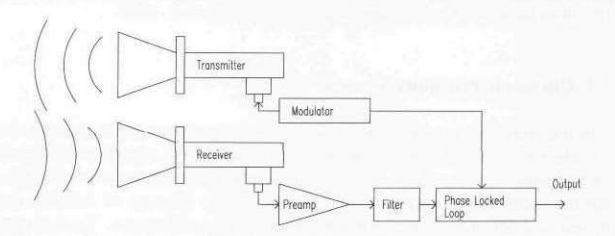
\includegraphics[scale=0.4]{figures/7_microwave_presence_sensor.png}}%
			{Fonte: \cite{hayward2022capaciflector}}
			\caption{O sensor de presença de microondas, requere uma antena transmissora e outra receptora separadas.}
			\label{fig:7_microwave_presence_sensor}
		\end{figure}
		\item Podem ser empregados na indústria automotiva, automação industrial e sistemas de segurança.
	\end{itemize}
\end{frame}

%------------------------------------------------
\section[Optical Proximity Sensors]{Optical Proximity Sensors} 
%------------------------------------------------
\begin{frame}[allowframebreaks, fragile]
\frametitle{Optical Proximity Sensors}
	\begin{itemize}
		\item São comumente encontrados em aplicações robóticas como:
		\begin{itemize}
			\item Detecção de piso;
			\item Referenciamento na navegação;
			\item Prevenção de colisão.
		\end{itemize}
		\item A energia modulada próximo do infravermelho é tipicamente empregada para reduzir os efeitos da iluminação ambiente, alcançando assim a relação sinal-ruído necessária para uma operação confiável \cite{everett1995sensors}.
		\item Sua performance depende de:
		\begin{itemize}
			\item Características físicas do material o qual se deseja estimar proximidade (tamanho, formato, refletividade e o tipo de material);
			\item Design do sensor;
			\item Velocidade do emissor ou do alvo;
			\item Qualidade e quantidade de energia erradiada/recebida.
		\end{itemize}
		
		\newpage
		\item \textit{Opposed Mode}:
		\begin{itemize}
			\item 
		\end{itemize}
		\begin{figure}
			\centering
			\copyrightbox[b]{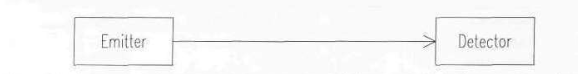
\includegraphics[scale=0.7]{figures/8_optical_sensor_opposed_mode.png}}%
			{Fonte: \cite{everett1995sensors}}
			\caption{\textit{Opposed Mode sensor configuration} depende da passagem de um objeto entre o transmissor e receptor para interomper o feixe.}
			\label{fig:8_optical_sensor_opposed_mode}
		\end{figure}

		\newpage
		\item \textit{Retroreflective Mode}:
		\textit{Opposed Mode}:
		\begin{itemize}
			\item 
		\end{itemize}
		\begin{figure}
			\centering
			\copyrightbox[b]{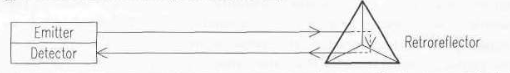
\includegraphics[scale=0.7]{figures/9_optical_sensor_retroreflective_mode.png}}%
			{Fonte: \cite{everett1995sensors}}
			\caption{\textit{Corner-cube retroreflectors} são empregados para aumentar o alcance efeitvo e simplificar o alinhamento dos feixes.}
			\label{fig:9_optical_sensor_retroreflective_mode}
		\end{figure}

		\newpage
		\item \textit{Diffuse-mode}:
		\begin{itemize}
			\item 
		\end{itemize}
		\begin{figure}
			\centering
			\copyrightbox[b]{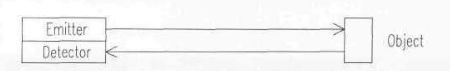
\includegraphics[scale=0.7]{figures/10_optical_sensor_diffuse_mode.png}}%
			{Fonte: \cite{everett1995sensors}}
			\caption{\textit{Diffuse-mode proximity sensors} dependem da energia refletida diretamente da superficie do alvo.}
			\label{fig:10_optical_sensor_diffuse_mode}
		\end{figure}

		\newpage
		\item \textit{Convergent Mode}:
		\begin{itemize}
			\item 
		\end{itemize}
		\begin{figure}
			\centering
			\copyrightbox[b]{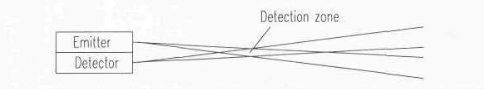
\includegraphics[scale=0.7]{figures/11_optical_sensor_convergent_mode copy.png}}%
			{Fonte: \cite{everett1995sensors}}
			\caption{\textit{Diffuse-mode proximity sensors} configurados em modo convergente podem ser usados para para determinar a distância aproximada de um objeto.}
			\label{fig:11_optical_sensor_convergent_mode}
		\end{figure}
	\end{itemize}
\end{frame}


%------------------------------------------------
%\section*{Referências}
%------------------------------------------------

\begin{frame}
    % \nocite{*}
    \printbibliography
\end{frame}


\begin{frame}
\titlepage % Print the title page as the first slide
\end{frame}

\end{document}